\section{NAX通证经济设计}
\subsection{设计目标}
设计公链的通证经济的目标除了更好的激活生态外,还需要在生态中起到积极正向的博弈作用。公链的通证经济的核心设计应当符合一定的原则和目标,例如:公平受益、正向激励、逻辑简洁,场景多样等。总而言之,公链的通证经济需要公正的获取场景和多样的消耗场景,使得通证拥有更高的持有价值,从而促进公链的发展和壮大,一个良好的公链通证经济,会使得整个生态变得更加有活力和动力。总结起来NAX的设计目标是:

\begin{enumerate}[\hspace{2cm}(a)]
    \item 公平受益
    \item 正向激励
    \item 简洁易懂
    \item 场景丰富
    \item 智能有效
\end{enumerate}

\subsection{核心逻辑}

\subsubsection{资产公平性与正当性}
公链通证经济的有效性的根本来自于资产获得的公平性和正当性。资产的获取规则应当简单透明,对绝大多数人应当是信息对称的。在公链的通证经济中,拥有的资产具有相对的公平性和正当性,因此通过质押(Staking)的方法作为获取通证权益的主要途径是符合要求的。不会因为规则不清晰,或者漏洞导致资产分配不理想的现象,并使得博弈的总体结果是有利于公链生态发展的方法。在星云的生态当中,质押(Staking)NAS,以获取相应的NAX权益,这在星云生态通证经济体内是公平公正的。

\subsubsection{星云式智能质押}
传统的质押方式是用户将资产转入到智能合约当中暂为保管,资产安全问题维系在一个智能合约里,合约资产安全性问题历史上屡见不鲜,2016年以太坊的The DAO攻击事件,攻击者利用了合约漏洞使得投资者产生巨大的经济损失,也使得投资者对合约安全性产生怀疑。另一方面,质押同时也给公链项目方带来非常大的压力,大量资产保存在一个合约当中,使得合约的管理及安全性成为一个非常大的发展瓶颈。区块链上的资产是确权的,质押(Staking)只是锁住流动性,并不是资产的确权性(虽然可以通过调用合约方法取回)转移到合约里。

通过设计NAX的机制,我们提出星云式质押(Nebulas Smart Staking),在确保用户资产的确权仍然属于用户的前提下,用户与质押合约签定的锁住流动性的契约记录在合约上。质押合约的作用只是通过链上随机检查契约的有效性来保持用户的质押有效性。当地址的余额大于等于契约的数额的时候,被认为是有效质押。星云式智能质押的优势是:
\begin{enumerate}[\hspace{2cm}(a)]
    \item 保证用户的资产确权
    \item 激励更多的用户参与质押
    \item 资产安全性去中心化
    \item 资产的确权性与锁住资产流动性分离
\end{enumerate}

\subsubsection{NAX增发模型 - NDM}
如上述提到的,在保障资产公平性与正当性基础上,确保用户质押资产所有权神圣不可侵犯的前提下,用户贡献出资产的流动性以获取相应的生态权益。我们称这种新式增发模式为NDM(Nebulas Devotion Mining)。NAX的预计发行总量上限是100亿(\(10^{10}\)。 增发周期为每6,000高度(一天左右),每周期增发数量呈递减规律,衰减系数$\mu=0.999$,预计12年左右发放完全。预增发NAX数量随周期数的变化图\ref{dist}所示,累积预增发NAX数量如图\ref{acc}所示。

\begin{figure}
\centering
    \begin{tikzpicture}
    \begin{axis}[
        axis lines = left,
        xlabel = {周期数},
        ylabel = {每日预发行NAX数量},
    ]
    \addplot [
        domain=-0:4000, 
        samples=1000,
        color=red,
    ]
    {1.0*10^7*0.999^x};

    \end{axis}
    \end{tikzpicture}
    \caption{每日预发行NAX数量与周期关系}\label{dist}
\end{figure}


%累积增发NAX数量与周期关系
\begin{figure}
\centering
    \begin{tikzpicture}
    \begin{axis}[
        axis lines = left,
        xlabel = {周期数},
        ylabel = {累积预增发NAX数量},
    ]
    \addplot [
        domain=-0:4000, 
        samples=1000, 
        color=red,
    ]
    {10^10*(1 - 0.999^(x+1))};

    \addplot [
        domain=-0:4000, 
        samples=1000, 
        color=blue,
    ]
    {10^10};
    \end{axis}
    \end{tikzpicture}
\caption{累积预增发NAX数量与周期关系}\label{acc}
\end{figure}

\subsubsection{动态分发模型}
所谓动态分发模式是指,在预增发的基础上,将引入有一些变量以促进生态的正向博弈,在NAX起初,我们引入质押率影响因子,根据质押率的涨跌,动态调整分发比例的大小,并将未分发的NAX滚动到下一个周期当中。以后根据需要,我们还将引入更具博弈色彩的动态分发模式。

因此,每个周期$i$, 系统会预增发 $C_i$ 个NAX分配给目前正在质押的用户。系统在实际分发的时候会根据当前的质押率水平 r(当前参与质押NAS的总量/总体NAS流通总量)确定一个分发系数$\lambda_i$, 实际分发 $C_i$$\lambda_i$ (0<$\lambda_i$<1)个NAX,剩余未分发的 $C_i$(1 - $\lambda$) 个NAX将滚动到下一个周期的预增发总量里面。因此,第\(i\)期增发池,\(C_i = C_0 \mu^i + C_{i-1} (1-\lambda_{i-1})\),包含两部分。第一部分为基础部分,每一期不断衰减,衰减系数$\mu$。第二部分为上一期增发池中的剩余部分。


其中,分发系数\(\lambda_i\)与质押率\(r_i\)的函数关系如以下公式所示,具体参数,请参看附录。其函数关系如图\ref{func}所示。

  \begin{equation}
    \lambda_i = l r_i^3 + m r_i^2 + n r_i
  \end{equation}

\begin{figure}
\centering
    \begin{tikzpicture}
    \begin{axis}[
        axis lines = left,
        xlabel = {质押率$r_i$},
        ylabel = {分发系数$\lambda_i$},
    ]
    \addplot [
        domain=0:1,
        samples=100,
        color=blue,
    ]
    {1.52*x^3-3.88*x^2+3.36*x};
    \addplot [
        domain=-0:1, 
        samples=100, 
        color=red,
    ]
    {1};
    \end{axis}
    \end{tikzpicture}
    \caption{分发系数与质押率的关系}\label{func}
\end{figure}



\subsubsection{周期内分配模型}
在一个分发周期内,不同的质押周期数将获得不同的分发权重。系统根据每个质押用户的质押数量$V_{i,j}$以及质押权重\(f(T_{i,j})\)决定最终所获得的NAX分发量。假如第$i$周期内,有$N$个地址正在有效质押,其中第$j$地址质押数量为$V_{i,j}$, 有效质押周期数为$T_{i,j}$。因此,该地址所能分发到的NAX数量$K_{i,j}$如以下公式所示。

\begin{equation}
  K_{i,j} = \frac{V_{i,j} f(T_{i,j})}{\sum_j V_{i,j} f(T_{i,j})} \lambda_i C_i
\end{equation}



其中,\(f(T_{i,j})\)是第\(i\)期用户\(j\)的质押的有效权重函数。质押权重与质押周期数的关系,如下公式所式,其中函数关系如图\ref{weight}所示。
  \begin{equation}
    f(T) = 1 - \frac{\sqrt{(aT+b)^2+c^2}-(aT+b)}{2}
  \end{equation}

公式中的参数$a$,$b$,$c$等将会在附录中讨论。总的来说,同一个周期内,系统会根据质押数量以及相应的质押时间长短来分配增发的总量,以达到公平的效果,即质押数量越多,质押时间越长,所分配到的增发数量也会更多。但同时使得让新进来的质押用户有更高的积极性,新用户的权重也会维系在一个可观的水平上。 该设计会达到以下博弈场景:

\begin{enumerate}[\hspace{1cm}(a)]
  \item 早期参与质押的用户,有更大的概率获得更多的系统增发
  \item 随着质押率增加,系统增发数量也会相应提高,以鼓励更多人加入质押
\end{enumerate}

\begin{figure}
\centering
    \begin{tikzpicture}
    \begin{axis}[
        axis lines = left,
        xlabel = {质押周期数},
        ylabel = {有效权重},
    ]
    \addplot [
        domain=0:365,
        samples=200,
        color=blue,
    ]
    {1-(sqrt((0.005*x-0.3)^2+0.2^2)-(0.005*x-0.3))/2};

    \addplot [
        domain=-0:365, 
        samples=200, 
        color=red,
    ]
    {1};
    \end{axis}
    \end{tikzpicture}
    \caption{质押的有效权重与质押周期数的关系}\label{weight}
\end{figure}

\subsubsection{基金会增发手续费}
为了使得星云基金会能在生态上进行更多的投资、孵化,扶持,活动等事项中有更多的空间和主动权,NAX的增发中将有$5\%$的增发比例会转到一个由基金会多签管理的地址当中,该地址也将受公众监督的,其用途也是公开透明的方式。具体的活动内容在将来会有披露。


\subsection{合约框架}
NAX是扩展性的NRC20合约,由一组合约组成,并配合多签合约管理整个合约里的数据和参数,详细如图\ref{fig:nax_framework}所示。

\begin{figure}[htbp]
  \centering
    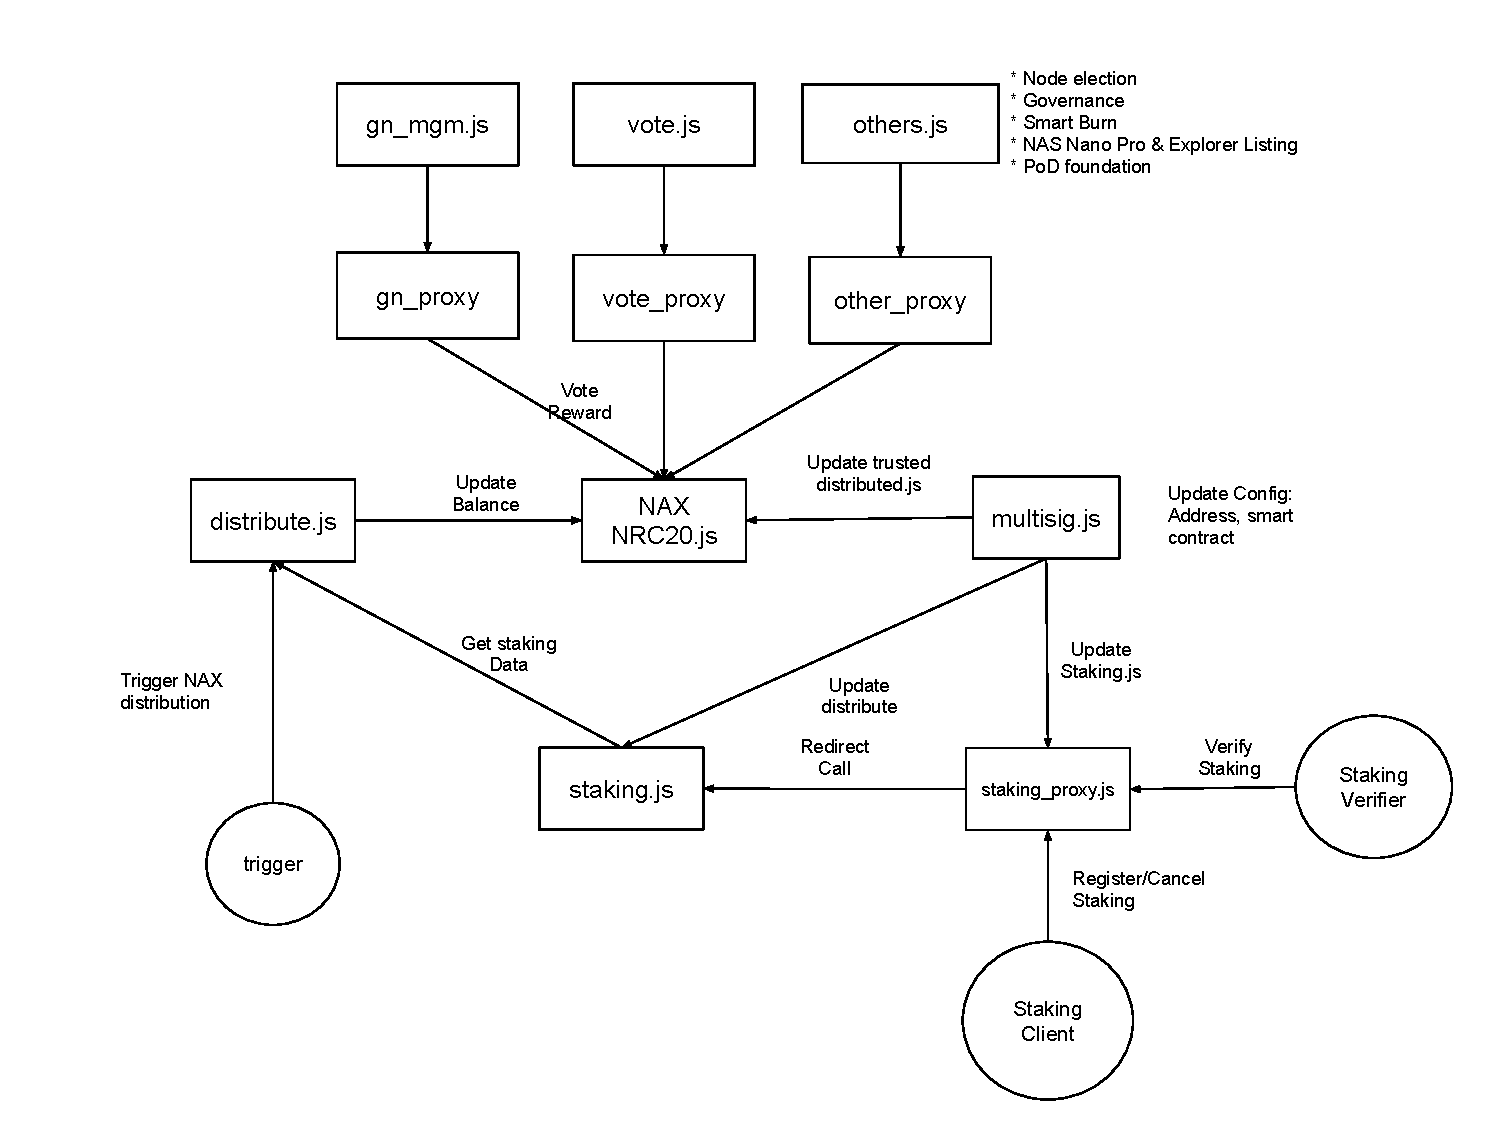
\includegraphics[width=1\textwidth]{../common/nax.pdf}
    \caption{NAX 合约组件示意图 \label{fig:nax_framework}}
\end{figure}
